\newchapter{2}{Глава 2}

\section{Контекстная информация}

Несмотря на удобство и простоту стандартных методов коллаборативной фильтрации, данная модель не содержит в себе огромное количество другой доступной информации, будем называть такую информацию \textit{контекстной}. Контекстной информацией может быть все что угодно, дата покупки (выходной или будний день), фанр фильма, возраст пользователя и так далее. Наличие такой информации должно повысить точность рекомендаций и их полезность. Так, например, на выходных можно рекомендовать фильмы для семейного просмотра, а по будням непродолжительные сериалы.

\section{Встраивания контекстной информации}

Cуществует несколько общих методов встраивания контекстной информации в рекомендательную систему.

\begin{itemize}
\item \textbf{Contextual Pre-Filtering}. Суть данного метода заключается в фильтрации не подходящих под текущий контекст оценок, дальше задача решается стандартными алгоритмами.

\item \textbf{Contextual Post-Filtering}. После нахождения списка рекомендаций стандартными методами, предметы, не подходящие под текущий контекст, удаляются.

\item \textbf{Contextual Modeling}. Контекстная информация встраивается на уровне модели. При таком способе встраивания контекстной информации, стандартные методы решения задачи о рекомендациях уже не работают или же требуется их адаптация.

\end{itemize}

В данной работе будет рассмотрен последний из методов, а именно, метод встраивания контекстной информации в матрицу отзывов.

\section{Контекстная информация в CF}

В работе будет использоваться набор данных MovieLens, он содержит отзывы на фильмы, а так же ряд дополнительной информации: возраст, пол и род деятельности пользователя, жанр и год выпуска фильма (один фильм может иметь несколько жанров).

Обозначим контекстную информацию, относящуюся к пользователю за $\mathcal{C_U}$, а к предметам за $\mathcal{C_I}$. 

\begin{gather*}
\mathcal{C_U} = {M, F, Job_1, ... , Job_{19}} \\
\mathcal{C_I} = {genre_1, ..., genre_{19}}
\end{gather*}
$$

К исходной матрице отзывов по строкам допишем информацию о предметах, а по столбцам информацию о пользователях, таким образом, матрица отзывов размера $m$ на $n$ примет размер $m+|C_I|$ на $n+|C_U|$. Если предмет или пользователь содержит контекстную информацию, то в соотвествующей ячейке матрицы ставится оценка 5, иначе 0.

\begin{figure}[H] 
\centering
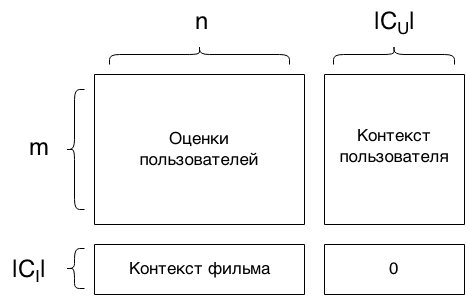
\includegraphics[scale=0.8]{CFContextMatrix.png}
\caption{Схема расширенной матрицы отзывов с контекстной информацией}
\label{fig :metka1}
\end{figure}

Таким образом мы получили $\mathit{расширенную матрицу отзывов}$, которая содержит в себе всю необходимую информацию. Отличие от стандартной матрицы заклюичается в том, что добавленные строчки, как бы являются пользователями, которые очень любят фильмы определенного жанра. Алгоритм CF учтет таких пользователей и найдет наиболее схожих с ними. Аналогичную аналогию можно провести и для добавленных столбцов. К новой матрице можно применить уже описанный ранее метод разложения SVD.